\documentclass[11pt,a4paper,headsepline,footsepline,bibliography=totocnumbered]{article}

\usepackage[utf8]{inputenc}
\usepackage{lmodern}
\usepackage[ngerman]{babel}
\usepackage[T1]{fontenc}
\usepackage[left=2.5cm,right=2.5cm,top=2.5cm,bottom=2.5cm]{geometry}
\usepackage{microtype}
\usepackage{bookmark}

\usepackage{fancyhdr}
\usepackage[onehalfspacing]{setspace}
\usepackage[font=small]{caption}


% Abb. statt Abbildung als Caption
\addto\captionsngerman{\renewcommand{\figurename}{Abb.}}
% Tab. statt Tabelle als Überschrift
\addto\captionsngerman{\renewcommand{\tablename}{Tab.}}

\setlength{\headheight}{14pt}

\usepackage{chngcntr}
\counterwithout{equation}{section}
\renewcommand{\theequation}{\arabic{equation}}

%change font
\renewcommand{\familydefault}{\sfdefault}

\usepackage{tikz} %Zum Diagramme zeichnen
\usepackage{pgfplots}
\pgfplotsset{compat=1.17}

\setlength{\parindent}{0cm} % Einrückung bei Paragraphenbeginn entfernen

%%%

\begin{document}
\pagestyle{fancy}
\pagenumbering{arabic}

\thispagestyle{empty}

\begin{center}
  \begin{figure}[h]
    
\includegraphics[width=5cm]{pictures/htw-logo.png}
  \end{figure}

  \vspace{0.25cm}

  \huge{HTW Berlin}
  \linebreak
  \Large{Fachbereich 4 - Informatik, Kommunikation und Wirtschaft}
  \linebreak
  \Large{BA - Angewandte Informatik}
  \linebreak

  \vspace{0.25cm}

  \textbf{\Huge{Semesterbegleitende Arbeit - KilterVote}}

  \vspace{0.25cm}

  \Large{B35 - Mobile Betriebssysteme und Netzwerke}
  \linebreak
  \large{WiSe - 24/25}
  \linebreak
  \large{Prof. Dr. Thomas Schwotzer}
\end{center}

\vspace{1cm}

% \begin{verbatim}
% \end{verbatim}

% \begin{verbatim}
% \end{verbatim}

\begin{flushleft}
\begin{tabular}{lll}
  \textbf{Bearbeitende:} & & Yannik Schüler \\ & & Simon Cornelius \\
  \textbf{Matrikelnummern:} & & 583880 \\ & &  577602 \\
\end{tabular}


\end{flushleft}

\pagebreak
\tableofcontents

\newpage

\section{Projektidee}

\subsection{Beschreibung}
  \par
    Die Applikation soll zum Voten von Routen am Kilter Board in einer Boulderhalle helfen.
    Denn oftmals ist es schwer eine unparteiische Wahl zwischen verschiedenen Schwierigkeitsgeraden der Routen zu gewährleisten, gerade wenn eine weite Spanne von Erfahrungsstufen unter den Boulderern vertreten ist.
    Jeder Boulderer kann Routen zu einem Pool hinzufügen und diese einem bestimmten Level zuordnen, dieses darf jedoch nie sein eigenes Level überschreiten.
    Dann kann jeder Boulderer für eine Route stimmen und ein Voting Algorithmus basierend auf den Erfahrungsstufen wählt dann eine Route aus.
    Während des Kletterns loggen die Boulderer ihre Versuche auf jeder Route um am Ende eine Auswertung zu erhalten.
    Auf Wunsch können die persönlichen Statistiken auch gespeichert werden, sowie Statistiken zwischen bestimmten Boulderern.
    Sessions bieten verschiedene Modifikationen, welche den Voting Algorithmus betreffen, sowie generelle Einstellungen der Session, wie die maximale Anzahl der Versuche pro Route.

\subsubsection{Use Cases}
  \begin{enumerate}
    \item Session erstellen oder einem Session beitreten durch Angabe eines Session Codes (möglicherweise auch via NFC)
    \item Angabe eines Namens und dem eigenen Erfahrungslevel im Bouldern
    \item Hinzufügen k/einer oder mehrerer Routen zum Route Pool
    \item Ansehen der verschiedenen Routen im Pool
    \item Voten für eine Route
    \item Loggen der Versuche mit Fortschritt (in Prozenten), sowie dem Erreichen eines Checkpoints
    \item Ändern des eigenen Erfahrungslevels während einer laufenden Session
    \item Ändern der Session Regeln während einer laufenden Session
  \end{enumerate}

\subsubsection{Use Case Diagram}

\subsection{Wireframes}
  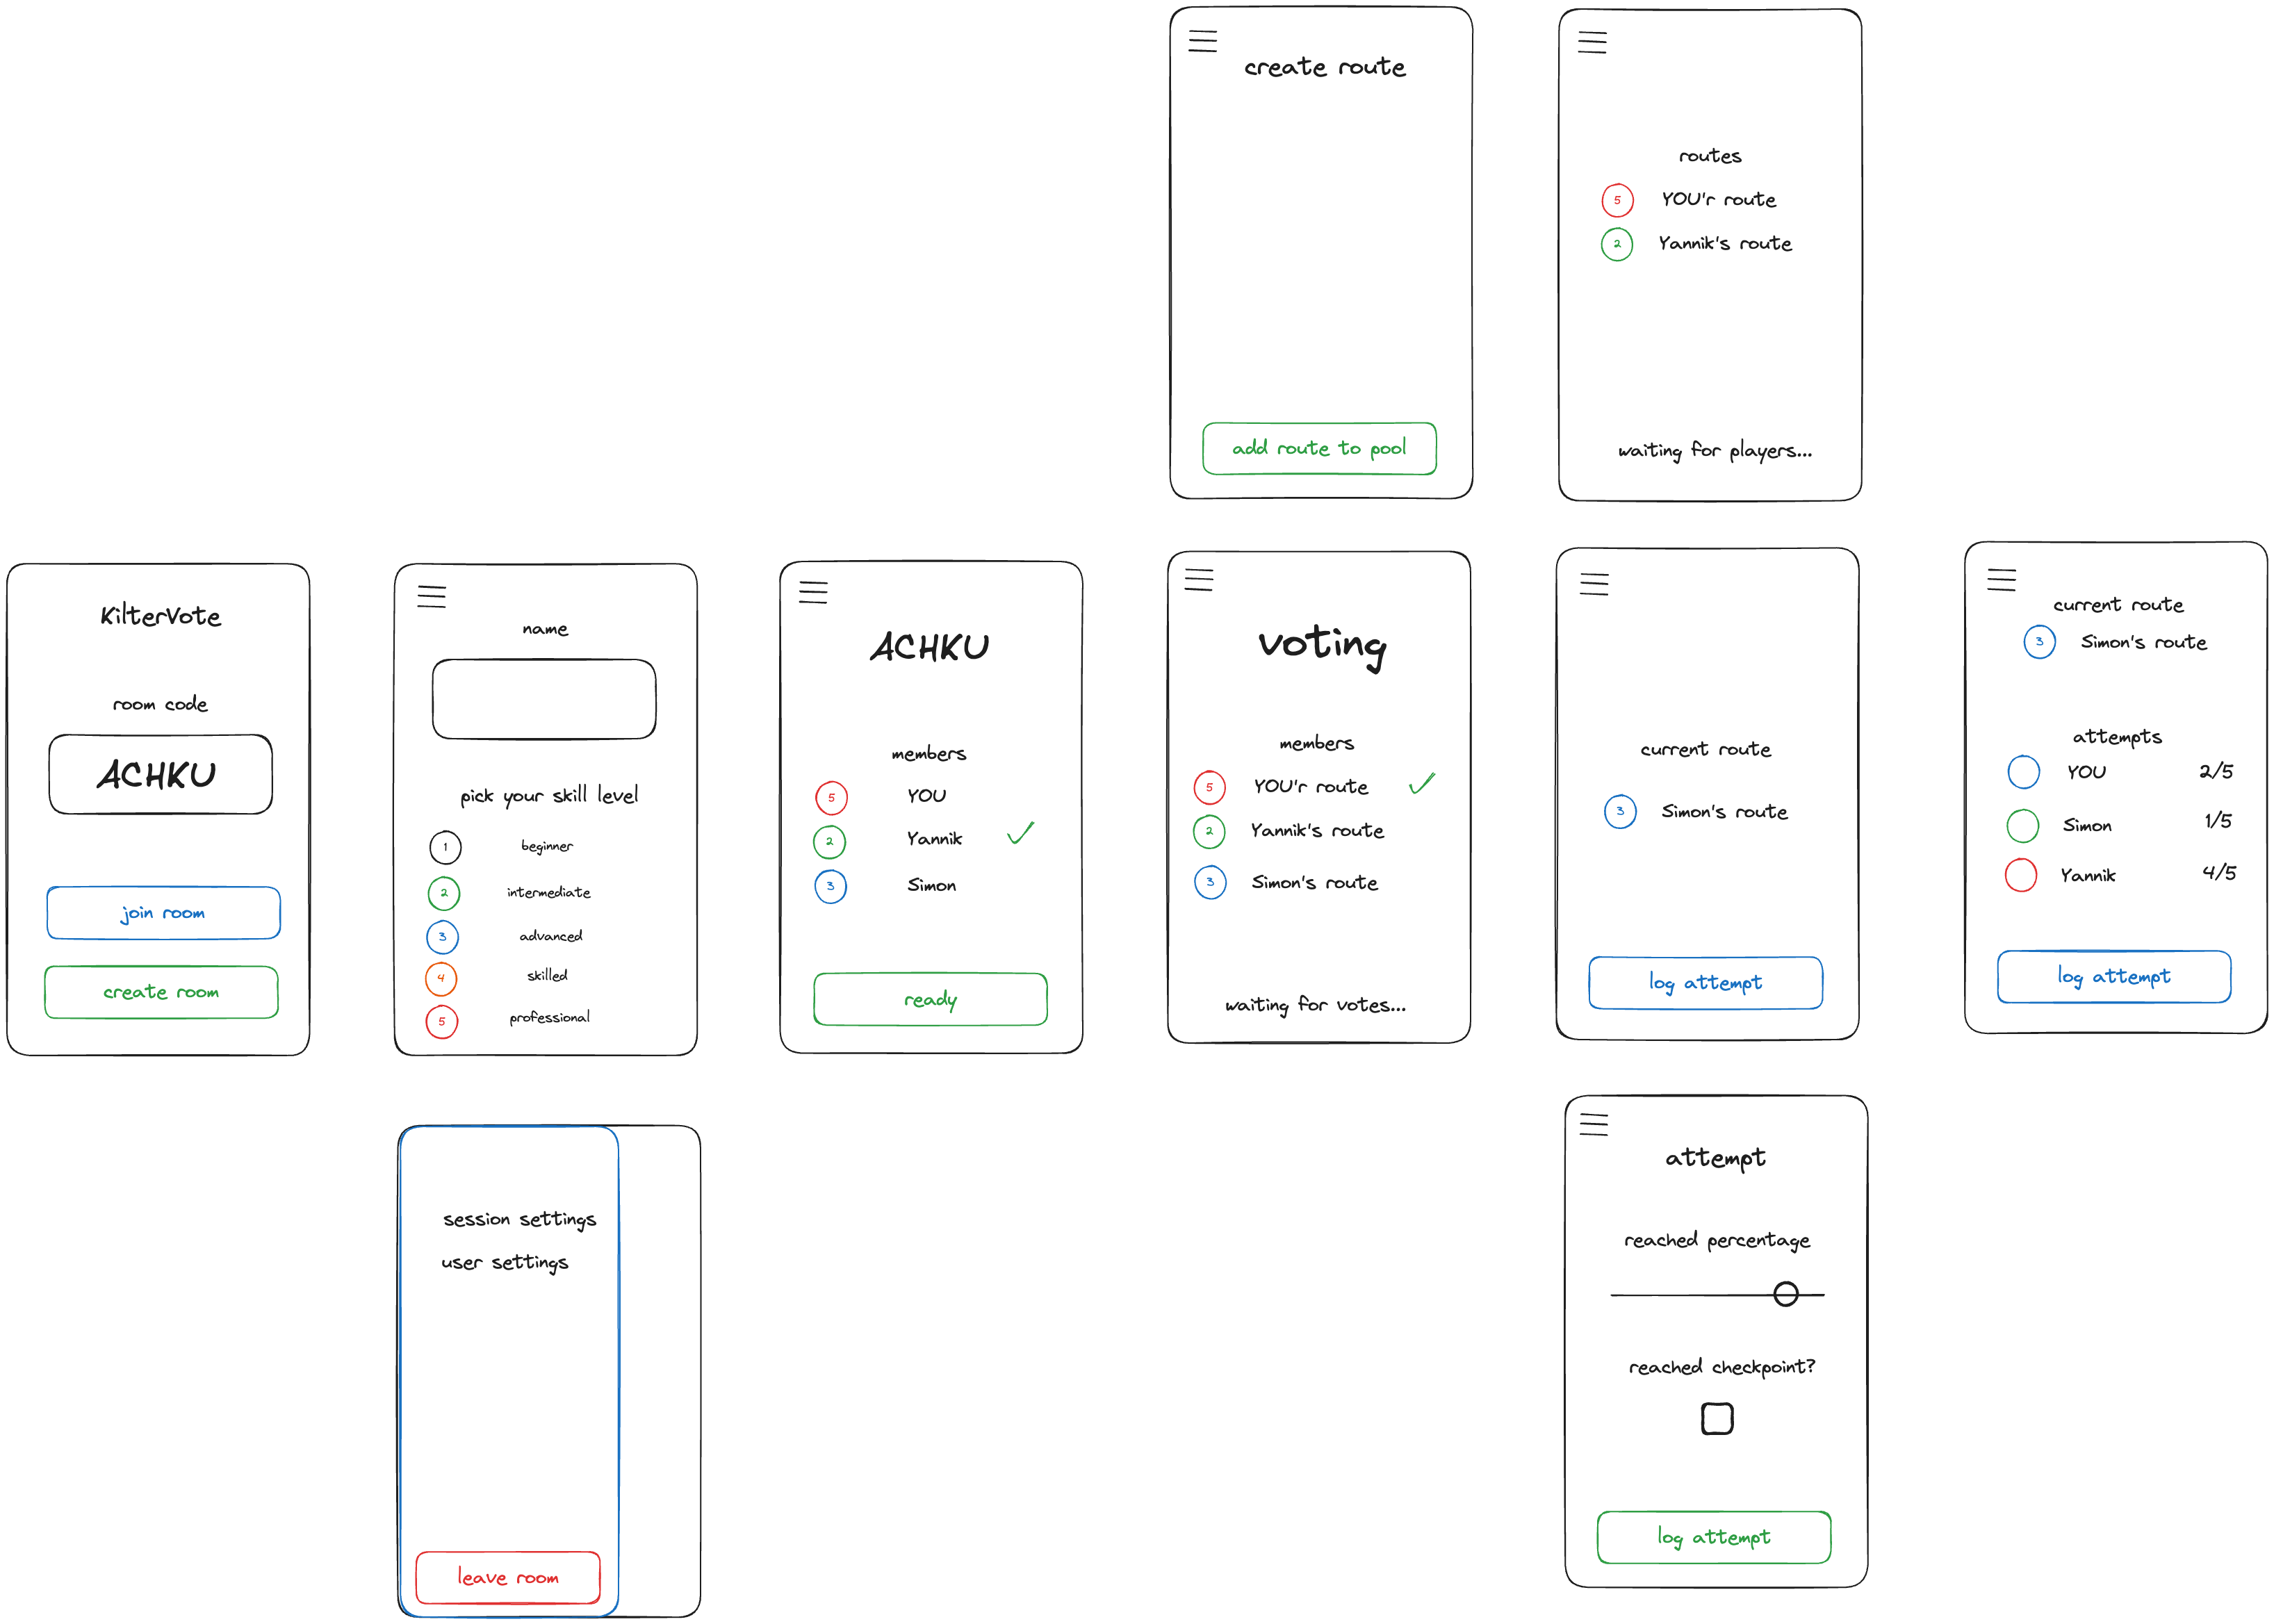
\includegraphics[width=\textwidth]{pictures/KilterVote_GUI.png}

\end{document}
